\documentclass[10pt,conference,compsocconf]{IEEEtran}

\usepackage[utf8]{inputenc}
\usepackage{hyperref}
\usepackage{graphicx}	% For figure environment


\begin{document}
\title{Machine Learning Course - Project 1}

\author{
  Quentin Laville, Valentin Moullet, Joël M. Fonseca\\
  \textit{Department of Computer and Communication Sciences, EPFL, Switzerland}
}

\maketitle

%%%%%%%%%%%%%%%%%%%%%%%%%%%%%%%%%%%%%%%%%%%%%%
\section{Introduction}

The whole process described here concerns the first project of the CS-433 Machine Learning class. The goal is to apply various machine learning models on a dataset provided by the CERN, generated by the Large Hadron Collider, in order to distinguish experiences resulting in background from Higgs boson decay.

%%%%%%%%%%%%%%%%%%%%%%%%%%%%%%%%%%%%%%%%%%%%%%%
\section{The Data}

\subsection{Provided}

Two datasets are given: a train and test set. The train set contains more than $N_1 = 250k$ experiences with outcomes (either a 'b' for background, and 's' for signal $-$ i.e., a Higgs boson decay). The test set contains more than $N_2 = 500k$ experiences without the outcome. Each sample was described by a row of $D = 30$ features.

\subsection{Pre-processing}

\subsubsection{Standardization}

We standardize both the training and the test sets using the training mean and variance.

\subsubsection{Dataset split}

After analyzing the data sets, one can notice that only one feature is categorical: $PRI\_jet\_num$ takes value in $[0,3]$. Moreover, some features seems to match a pattern following this $jet$ number. Thus, data points having $jet=0$ miss a lot of values, the same when $jet=1$ but in a lesser proportion and when $jet=2$ or $jet=3$, the vales for the features are almost complete (as well as being quite correlated). After this exploration, we decided to train the data points that have different $jet$ numbers separately, as they look like different in nature.

\subsubsection{Missing values}

As experiences could not always give relevant data, missing values ($-999.0$) were filled with a $NaN$ values. As we have seen above, some features don't make sense anymore for some $jet$ values, hence they are removed. For the others, the $NaN$ values are replaced by the median of the corresponding column.

\subsubsection{Feature engineering}

%%%%%%%%%%%%%%%%%%%%%%%%%%%%%%%%%%%%%%%%%%%%%%%%
\section{Machine Learning Models and Methods}

\subsection{Models}

The following models were used throughout the project:

\begin{enumerate}
\item Gradient descent ($\gamma$, $iterations$)
\item Stochastic gradient descent ($\gamma$, $iterations$)
\item Least square with a polynomial basis ($degree$)
\item Ridge regression with a polynomial basis ($degree$, $\lambda$)
\item Logistic ($degree$, $iterations$, $\gamma$)
\item Regularized logistic regression ($degree$, $iteration$, $\gamma$, $\lambda$)
\end{enumerate}

All the parameters inside the parentheses are exhaustively tested by grid search. 

\begin{enumerate}
\item $iterations \in \{50, 100, ... , 1000\}$
\item $degree \in \{1, 2, ... , 15\}$
\item $\gamma \in \{0.05, 0.1, ... , 1.0\}$
\item $\lambda \in \{1\mathrm{e}{-4} ... , 1\mathrm{e}{-1}\}$
\end{enumerate}

Note that the last parameter is computed in logarithmic space.

\subsection{Cross validation}

To train and test the different models, the 10-fold cross validation is used. This technique consists in splitting the data set in 10 size-equivalent bins. Then each bin is selected as the test bin, one after the other, and the 9 remaining ones are used to train the model. When the model is ready, you can check its validity again the test bin. This is helpful to avoid the over-fitting of a particular model over the training set.

\subsection{Accuracy estimation}

To compute accuracy, we simply computed the ratio between the resulting $y_{train}$ and the true $y$. By the 10-fold cross validation, the final accuracy was done by doing the mean of each $y_{train}$ obtained for each iteration. On top of that, we also computed the variance in order to show that the accuracy is indeed stable or not among the different folds.

\subsection{Best Model}

After using all models created with all related parameters with grid search, ridge regression give the best results. It's quite surprising, as we expect the logistic models to win this round, the problem being a classification problem (tell if a sample results in a Higgs boson decay or not). Note that the balancing of the train dataset isn't helping the overall accuracy against the test set, which could mean that the proportion is the same in the latter.

%%%%%%%%%%%%%%%%%%%%%%%%%%%%%%%%%%%%%%%%%%%%%%%%%
\section{Results}

\subsection{Figures and Tables}


\begin{figure}[tbp]
  \centering
  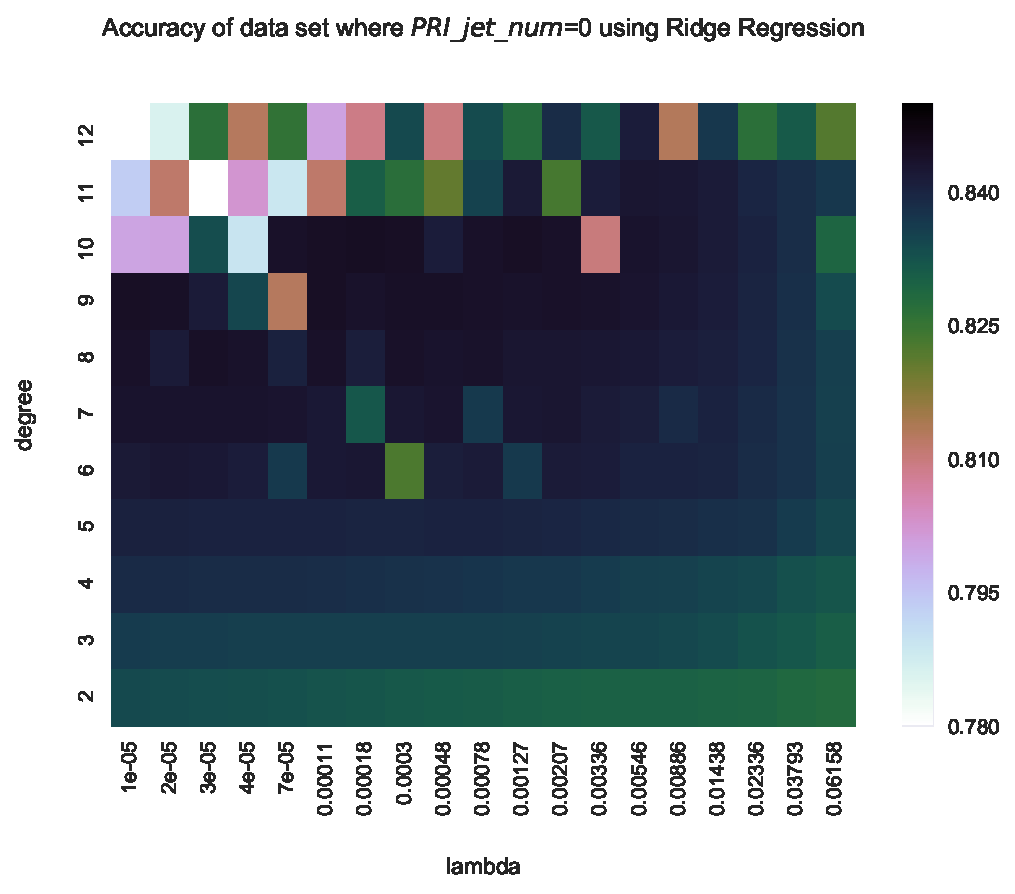
\includegraphics[width=\columnwidth]{figures/0_ridge_regression_black_version}
  \caption{Some test.}
  \vspace{-3mm}
  \label{fig:denoise-fourier}
\end{figure}
\begin{figure}[htbp]
  \centering
  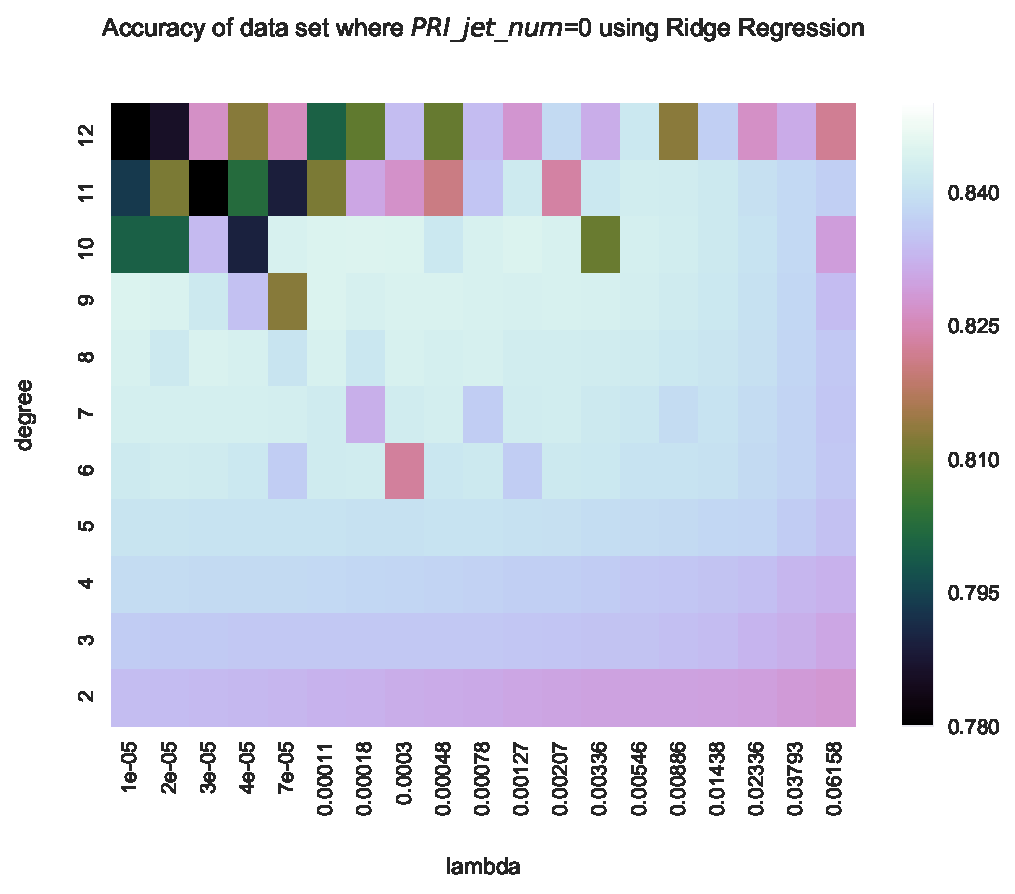
\includegraphics[width=\columnwidth]{figures/0_ridge_regression_white_version}
  \vspace{-3mm}
  \caption{Another test.}
  \label{fig:denoise-wavelet}
\end{figure}


\end{document}